\documentclass[11pt]{article}
\usepackage[utf8]{inputenc} % Para caracteres en espa�ol
\usepackage{amsmath,amsthm,amsfonts,amssymb,amscd}
\usepackage{multirow,booktabs}
\usepackage[table]{xcolor}
\usepackage{fullpage}
\usepackage{lastpage}
\usepackage{enumitem}
\usepackage{multicol}
\usepackage{fancyhdr}
\usepackage{mathrsfs}
\usepackage{pdfpages}
\usepackage{wrapfig}
\usepackage{setspace}
\usepackage{esvect}
\usepackage{calc}
\usepackage{multicol}
\usepackage{cancel}
\usepackage{graphicx}
\graphicspath{ {pictures/} }
\usepackage[retainorgcmds]{IEEEtrantools}
\usepackage[margin=3cm]{geometry}
\usepackage{amsmath}
\newlength{\tabcont}
\setlength{\parindent}{0.0in}
\setlength{\parskip}{0.05in}
\usepackage{empheq}
\usepackage{framed}
\usepackage[most]{tcolorbox}
\usepackage{xcolor}
\colorlet{shadecolor}{orange!15}
\parindent 0in
\parskip 12pt
\geometry{margin=1in, headsep=0.25in}
\theoremstyle{definition}
\newtheorem{defn}{Definition}
\newtheorem{reg}{Rule}
\newtheorem{exer}{Exercise}
% Two more packages that make it easy to show MATLAB code
\usepackage[T1]{fontenc}
\usepackage[framed,numbered]{matlab-prettifier}
\lstset{
	style = Matlab-editor,
	basicstyle=\mlttfamily\small,
}
\newtheorem{note}{Note}
\begin{document}  
\setcounter{section}{0}
\thispagestyle{empty}

\begin{center}
{\LARGE \bf Homework 3}\\
{\large AE370 - Spring 2018 \\ Emilio R. Gordon}
\end{center}
\vspace{20mm}
\textbf{Problem:} For the systems of equations 
\begin{equation*}
\begin{aligned}
5x_1-15x_2-x_3+2x_4 = 11 \\
3x_1+20x_2+4x_3 = -8 \\
x_1+6x_2+11x_3-3x_4 = 7 \\
4x_1+11x_2+3x_3+12x_4 = 4 \\
\end{aligned}
\end{equation*}
Solve the equations using the Jacobi method and the Gauss-seidel method. Stop when the system residual is of the same order of magnitude as the corresponding "exact solution" from Matlab's operator

\textbf{Solution:} 

The Jacobi Method converges within a tolerance of 1e-05 after the 30 iteration with a final solution u=[0.2159 -0.6594 1.1352 0.5820]

The Gauss-Seidel Method converges within a tolerance of 1e-05 after the 14 iteration with a final solution u=[0.2159 -0.6594 1.1352 0.5820]

The Matlab Function $A \textbackslash B = u$ has the final solution of u=[0.2160 -0.6594 1.1352 0.5820]

As we can see, both methods converged to the Matlab "exact" value. Note that the Gauss-Seidel method converges in almost half the number of iterations needed for the Jacobi method.

The following code was utilized to arrive at these solutions. Following the code are two plots. The first is the relative error of the magnitude of u compared for each method to the exact solution. The second plot is the convergence of each method looking at their residue.
\begin{figure}[H]
\begin{lstlisting}
function hw3
    tol = 0.00001;                                  % Tolerance
    A = [5 -15 -1 2; 3 20 4 0; 1 6 11 -3;4 11 3 12];% A Matrix defined by problem statement
    B = [11; -8; 7; 4];                             % B Matrix defined by problem statement
    exact = A\B;                                    % Exact Matlab Solution
    [uJ iterationsJ] = jacobi(A,B,tol);             % Run Jacobi Function
    [uGS iterationsGS] = gaussSeidel(A,B,tol);      % Run Gauss-Seidel Function
    plotter(A,B,tol)                                % Run Plotter Function
end
function [uJ iterations] = jacobi(A,B,tolerance)
    u = [0;0;0;0]; 
    M = zeros(size(A));
    N = -A;                  % Negative A
    for i=1:size(A,1)
        M(i,i) = A(i,i);     % Diagonal A
        N(i,i) = 0;          % Zero Diagonal Components
    end
    i = 0;
    while norm(B-A*u)>tolerance
        i=i+1;
        u = inv(M)*(B+N*u); % u_k+1 = M^-1 [B+N*u^k]
        iterations(i) = i;
        uJ(1:4,i) = u;
    end
end
function [uGS iterations] = gaussSeidel(A,B,tolerance)
    u = [0;0;0;0]; 
    M = triu(A);       % M is the Triangular Upper Bound of A
    N = M-A;           % N is the Triangular Lower Bound of A
    i = 0;
    while norm(B-A*u)>tolerance
        i=i+1;
        u = inv(M)*(B+N*u); % u_k+1 = M^-1 [B+N*u^k]
        iterations(i) = i;
        uGS(1:4,i) = u;
    end
end
function plotter(A,B,tol)
    [uJ iterationsJ] = jacobi(A,B,tol);
    [uGS iterationsGS] = gaussSeidel(A,B,tol);
    for j=1:length(uGS)
        GSRE(j) = norm(uGS(:,j)-(A\B))/norm(A\B);  % Compute Relative Error
        GSresidue(j) = norm(B-A*uGS(:,j));         % Compute Residue
    end
    for k=1:length(uJ)
        JRE(k) = norm(uJ(:,k)-(A\B))/norm(A\B);       % Compute Relative Error
        Jresidue(k) = norm(B-A*uJ(:,k));              % Compute Residue
    end
    plot(iterationsGS, GSRE,'LineWidth',2)
    hold
    plot(iterationsJ, JRE,'LineWidth',2)
    semilogy(iterationsGS,GSresidue,iterationsJ,Jresidue,'linewidth',2)
    %Significant Plotting Code removed for space
end
\end{lstlisting}
\end{figure}
\includepdf{plots.pdf}
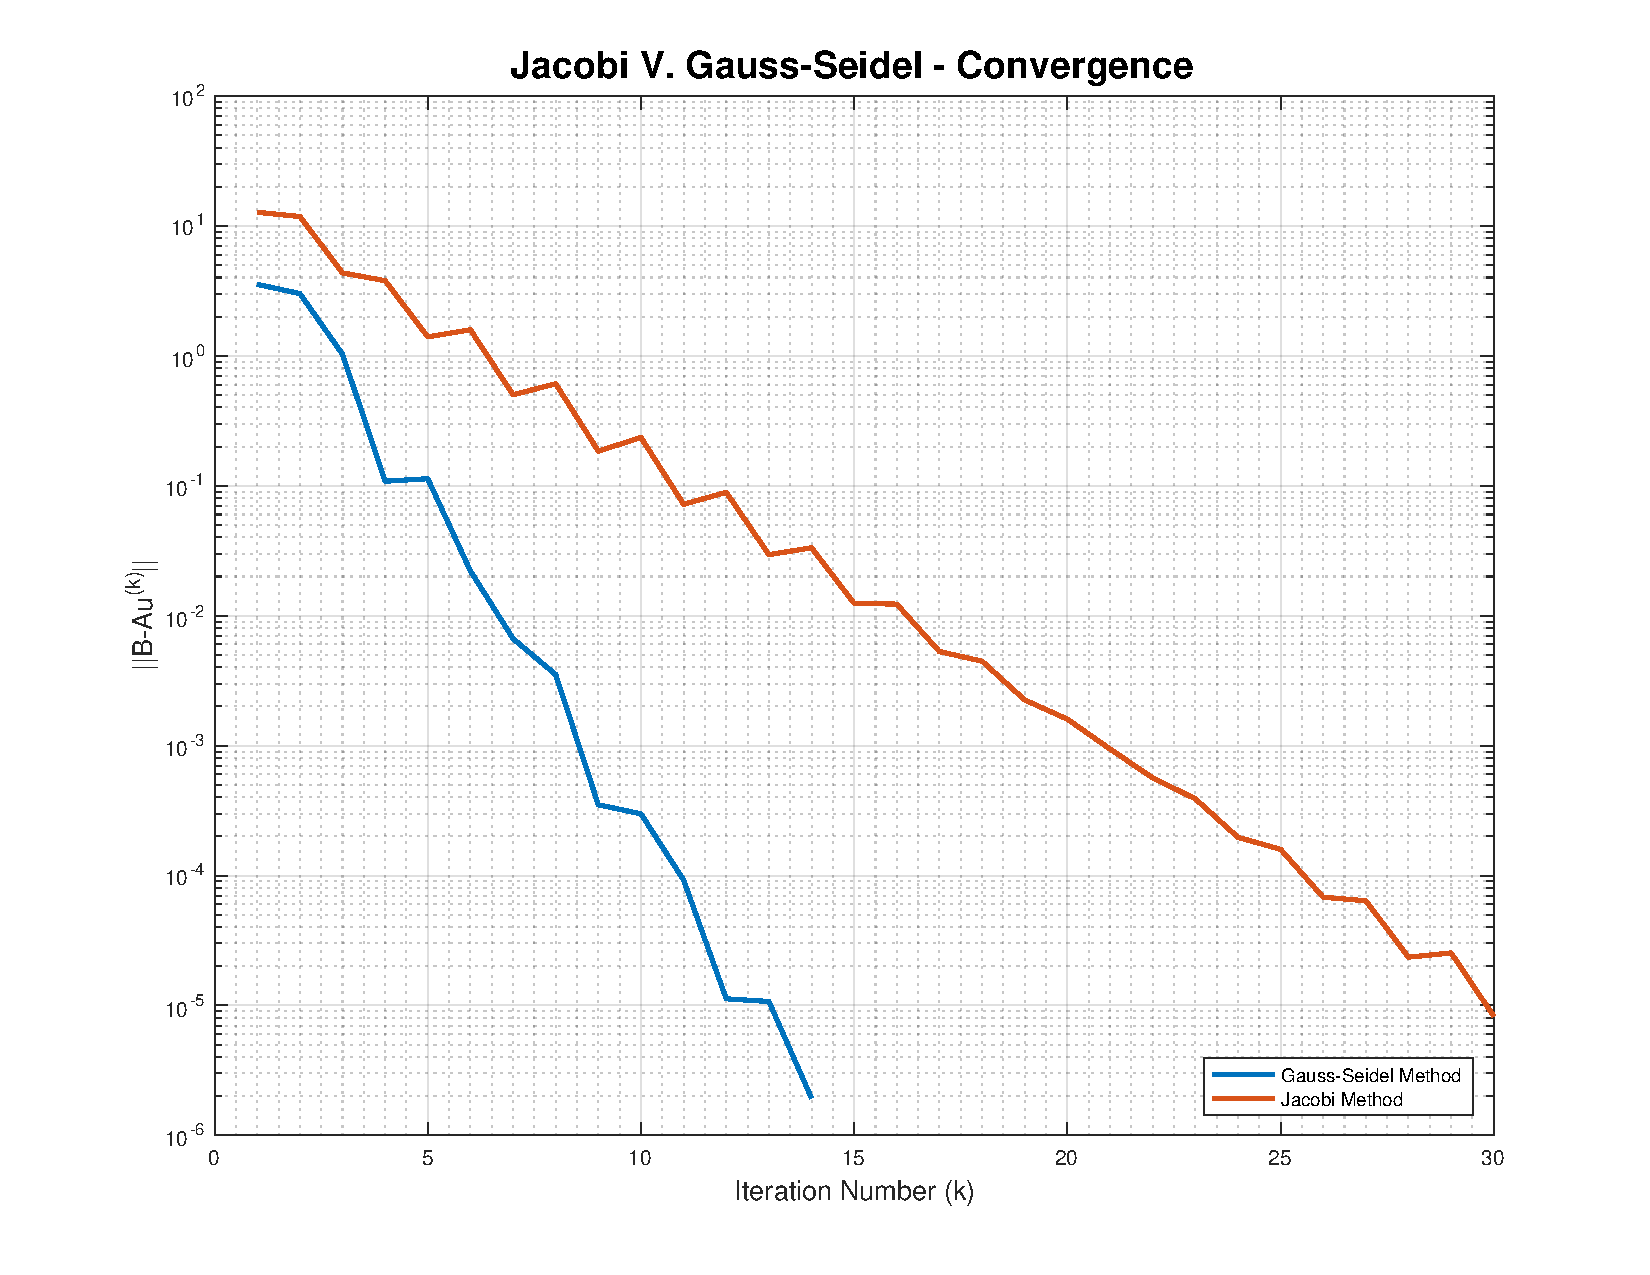
\includepdf{plots2.pdf}
\end{document}